\documentclass[12pt]{article}

% Set border
\usepackage[margin=1in]{geometry}

% Used for improving math typesetting and including certain symbols
\usepackage{amsmath}
\usepackage{physics}

% Use pictures and graphics
\usepackage{graphicx}
\graphicspath{ {images/} }

% Custom link colors
\usepackage{xcolor}
\usepackage{hyperref}
\hypersetup{
  colorlinks,
  linkcolor={black},
  citecolor={black},
  urlcolor={blue!80!black}
}

% Allow text to wrap around figures
\usepackage{wrapfig}

% Auto begin/end quotes (instead of having to use `` ")
\usepackage [autostyle, english = american]{csquotes}
\MakeOuterQuote{"}

% Used to include certain symbols (including /degree)
\usepackage{gensymb}

% Code listings/highlighting
\usepackage{minted}[cache=false]

% Allow subfigures (\subfloat, etc)
\usepackage{subcaption}

% TITLE ----------

\title{CMPU-250: Final Project Write-up \\
  \large Autonomous Robotics Design Competition Simulation}
\date{May 2018}
\author{George Witteman}

% DOCUMENT -------

\begin{document}

\maketitle

\begin{abstract}
  For my final project, I chose to design and implement an agent-based model of Vassar's Autonomous Robotics Design Competition class in the Cognitive Science department. This model simulates two robots in the arena using a slightly modified version of the real competition rules. The model is validated by testing individual functions for correctness, as well as visually testing that the behavior is correct. Finally, the model is evaluated using hypothesis testing to test assumptions about the competition, such that the addition of a camera will improve the efficiency of the robots or that increasing the velocity or rotation speed of the robot will increase it's score.
\end{abstract}

\section{Introduction}

Vassar's Autonomous Robotics Design Competition is a class in the Cognitive Science department that gives students the opportunity to create robots designed to complete a specific task. In the course, students work in teams and, using Arduinos, foam core, 3D printers, \href{http://charmedlabs.com/default/pixy-cmucam5/}{Pixy} camera, and various other electronics, build a robot that competes with the other team's robot to fulfill a certain task as best as possible within a given time frame.

This year, the goal of the competition is for teams to create a robot that gains the best score by collecting blocks of it's own quadrant's color into it's home quadrant, and removing blocks of other colors from it's home quadrant. There is also a sabotage element that can be implemented by moving blocks that are not the opponents color into the opponents quadrant.

During the actual competition, three of the four teams used a strategy that collected one block at a time and moved it to a different quadrant. My team decided that a collection strategy would prove more beneficial, since it could rely less heavily on the camera if that proved to not be easy to implement. Since we were not able to fully finish completing our robot, I wanted to build this model in order to test some of the theories we had to prove that a fully-implemented version of our robot would perform well.

This model includes a visualization of the arena that can be seen over time. See Figure \ref{fig:arena-1} for an example. In this figure, you're able to see the arena, including the outer and quadrant boundary lines, blocks, and robots. The two robots are represented by rectangles with a triangle in the middle to indicate their direction. The robots camera is also represented by drawing it's field of view as a mostly transparent semi-circle in front of the robot. The time that the simulation has been running for is indicated in the title of the plot, and when the simulation finishes the points for each team and winner is displayed in the MATLAB command window.

\begin{figure}[hbt]
  \center
  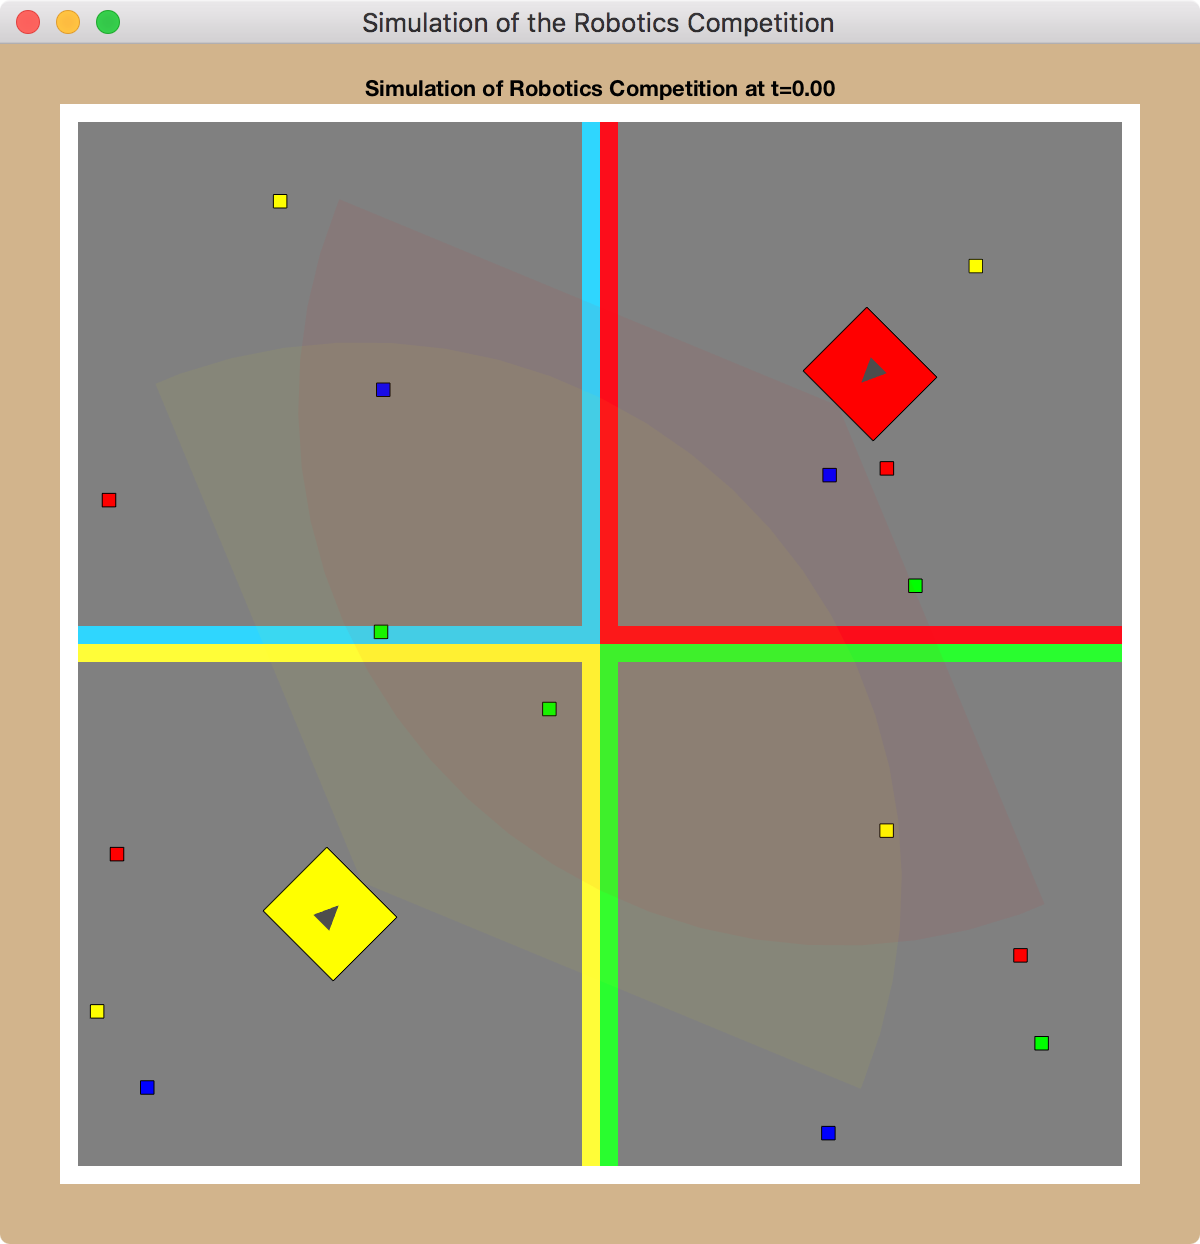
\includegraphics[width=0.7\textwidth]{images/arena-1.png}
  \caption{An example starting simulation state. You can see two robots (red and yellow) and twelve blocks spread out evenly through the four quadrants. The direction the robot is facing as well as it's camera's field of view is also represented.}
  \label{fig:arena-1}
\end{figure}

\section{Simplifying Assumptions}
This model is a fairly accurate representation of the actual competition. I chose to make the following simplifying assumptions to make the model simpler to implement.

\begin{itemize}
  \item Robots can reach their full velocity and stop instantly. In the real competition our robot could not speed up or stop instantly, so we gave the servos a 200ms time to allow the robot to come to a full stop before backing up. In this simulation we assume that our servos are perfect and the robot can go from full forward speed to full reverse speed instantly.
  \item All robots are identical in their software and hardware implementations. This is obviously not true in the real competition, but since we are just looking at analyzing a single implementation of the robot this is a reasonable assumption.
  \item The sorting mechanism is perfect. That is, blocks are either completely ignored (not moved at all) or collected into the chamber with 100\% accuracy.
  \item Blocks cannot be pushed, only collected or ignored. Again, this would not happen in the real competition. The assumption that we are making here is that given enough time we could devise a sorting mechanism that does not accidentally move blocks out of bounds or into a different quadrant.
  \item Placing blocks into the quadrant of the opponent or removing other color blocks from the home quadrant is insignificant. That is, being able to collect home color blocks and bringing them back to the home quadrant is the most important thing. We make this assumption in order to simplify the implementation, and under the observation that during the actual competition no robots got perfect scores.
  \item The robot's cameras are perfect accurate within their field of view. Here we're assuming that with enough time we'd be able to calibrate the colors on the camera to work well enough so that the robot could identify blocks at a high accuracy.
  \item A block that's at 0\degree\ vs 45\degree\ does not make a significant difference to our sorting mechanism. That is, the rotation of the blocks is insignificant and we can model all blocks as being placed in the arena at 0\degree.
  \item Robots can run over each when backing up, but not when going forward. I chose to make this assumption in order to prevent bots from getting stuck when they are backing up. This would mostly happen when $dt$ is low, and does not seem to impact the results of a simulation.
\end{itemize}

\section{How the Model Works}
This model is implemented in MATLAB using an object-oriented programming paradigm. I chose to use an object-oriented style, because I thought that it would keep the code clean, help with readability, make the code less prone to errors, and make it easier to debug. Since the model uses multiple physical "objects", I thought that mapped well onto this sort of code structure.

There is one \texttt{main.m} file that is responsible for setting the simulation parameters and running the simulation loop. From there, the \texttt{Arena.m} file implements the \texttt{Arena} class. The \texttt{Arena} class is in charge of integrating all of the other pieces of the simulation, including the \texttt{Block} and \texttt{Robot} classes. The \texttt{Robot} simulates each individual robot, and uses the \texttt{Camera} class to include the functionality of the camera, depending on a simulation parameter. There's also a \texttt{SimulationParameters} class that has properties for each parameter of the simulation. This class makes it easy to have all of the simulation parameters in \texttt{main.m} and pass those around to all the other classes that need them.

Each class (except \texttt{SimulationParameters}) has a \texttt{draw} function that is in charge of drawing the current frame on to the screen. The \texttt{Arena} and \texttt{Robot} classes also have a \texttt{nextFrame} function that update the next frame of the simulation. This is called once for each time step.

One important piece of the implementation that is used in many places throughout the code is the way that I represented the different shapes and detected when they collided or overlapped. To implement the functionality for this, I used the \texttt{polyshape} class in MATLAB. This class can create and plot any polygon onto the graph, and there are also a lot of useful functions that manipulate \texttt{polyshape}s.

For example, in order to detect when the center of a block was "underneath" a robot, I used the \texttt{isinterior} function. This function checks to see if a specific $(x,y)$ point is within a given \texttt{polyshape}. Another function that was used was the \texttt{overlaps} function. This function checks whether two \texttt{polyshape}s overlap, and was used for things such as checking whether the robots hit eachother.

In order to use these \texttt{polyshape}s in an efficient way, each class has a function that generates the \texttt{polyshape} for the entity at the given time. This can be used in situations like those in the previous paragraph, or to just be displayed to the screen.

To display the different entities to the screen, each class has a \texttt{draw} function which will plot the \texttt{polyshape} and possibly other information onto the graph. Since this can add to the total time needed to run the simulation, the simulation can be set to only show the first and last frames by changing the \texttt{drawArena} variable to \texttt{false} in \texttt{main.m}.

\subsection{Camera Implementation}
The main functionality of the camera is implemented in the \texttt{Camera} class. The constructor for this class takes as inputs the parameters for the camera, including the maximum distance that it can see objects, the maximum angle of it's field of view, the color of blocks that it should try to detect, and a flag indicating whether the camera should be turned on or not. 

Similar to the implementation of the other objects in the simulation, the \texttt{Camera} class uses \texttt{polyshape}s and the \texttt{isinterior} function to check if blocks are within the camera's field of view. It first creates a circle with a radius of the camera's maximum view distance and a triangle with the right position and angle. The usable field of view is then calculated by doing an intersection of those two shapes which gives the proper FOV angle and a consistent radius. Points can then be checked if they are in the interior of that resulting shape.

\begin{listing}[ht]
\begin{minted}[linenos]{matlab}
function ang = getAngleOffCenter(cam_x, cam_y, cam_R, obj_x, obj_y)
  %GETANGLEOFFCENTER
  % Calculate the angle of the object relative to the center
  % axis of the camera.
  cam_x2 = cos(deg2rad(cam_R)) + cam_x;
  cam_y2 = sin(deg2rad(cam_R)) + cam_y;
  
  if Camera.Debug
    plot([cam_x cam_x2], [cam_y cam_y2]);
    plot([cam_x obj_x], [cam_y obj_y]);
  end
  
  % Find the angle between the two lines created by the points
  ang = rad2deg(atan2(obj_y-cam_y, obj_x-cam_x) - ...
    atan2(cam_y2-cam_y,cam_x2-cam_x));
  
  % Correct for error
  if ang > 180
    ang = ang - 360;
  end
end
\end{minted}
\caption{The \texttt{Camera.getAngleOffCenter()} method.}
\label{lst:getAngleOffCenter}
\end{listing}

\subsection{States/Motion}
When the camera is not in use the motion is implemented simply. Robots start in the \texttt{State\_Drive} state (i.e. their \texttt{State\_Drive} property is set to \texttt{true}). Then they just move forward until they either hit another robot (\texttt{Arena.robotsHit()}), or have reached a boundary (\texttt{Robot.inBounds()}). If either of those conditions are true, then the robot goes into a spin-backup state, represented by setting the properties \texttt{State\_Spin} and \texttt{State\_Backup} to \texttt{true}. When this state is set to true, the \texttt{StateTime} property is also set to the number of seconds that we want to be in this state for. In this case, \texttt{StateTime} is set equal to \texttt{BackupTime}.

Once the robot is in the spin-backup state, it will backup for \texttt{BackupTime} seconds, decreasing \texttt{StateTime} by $dt$ every time step until \texttt{StateTime} equals zero. Once \texttt{StateTime} equals zero, the \texttt{State\_Backup} flag gets set to \texttt{false}, and we enter the spin state, with \texttt{StateTime} equal to a random number of seconds between $\texttt{MinSpinAngle} / \texttt{RotationSpeed}$ and $\texttt{MaxSpinAngle} / \texttt{RotationSpeed}$. What this means is that the robot will spin until the angle that it has spun is within \texttt{MinSpinAngle} and \texttt{MaxSpinAngle}.

If the camera is turned on, however, the behavior in \texttt{State\_Drive} changes. The robot will first check to see if there are any blocks in the field of view of it's camera. If there are, it finds the closest one, spins slightly towards it, and continues moving forward. The angle of spin per time step ($\frac{dR}{dt}$) is computed with the following equation, where $d$ is the angle (in degrees) of the block off the center axis of the camera and \texttt{Camera.ViewAngle} is the angle of the camera's field of view:

\begin{equation}
  \frac{dR}{dt} = (\texttt{RotationSpeed} \times dt) \times \frac{d}{\abs{d}} \times \frac{\sqrt{\abs{d}}}{\sqrt{\texttt{Camera.ViewAngle}/2}} .
\end{equation}

The first term in this equation gets the maximum number of degrees that the robot can rotate in a given time step. The second term sets the sign of the rotation (i.e. whether it should go left or right). The final term sets the proportion of the maximum degrees of rotation that the robot should move in this time step. It uses the square root in order to smooth out the turning, that is, to turn faster when the block is far away from straight in front of the camera, and to turn slower when it's almost directly in front of the camera. The reason that we want it implemented this way is to make sure that the robot is not darting left and right when the integration time of the camera (or $dt$ in the model), which is important on the real robot, is slow.

Finally, the robot will stop moving when it's back into it's home quadrant and either has all four blocks or has reached a given time limit, set by the simulation parameter \texttt{HomeStopTime}.

\subsection{Limitations}
There are some limitations to this implementation. One notable limitation is that the simulation runs very slowly because it has to generate the \texttt{polyshape} for each object in the simulation at least once per time step. This could be made less significant by only generating the \texttt{polyshape} once, and then applying transforms to it over time. However, this implementation was chosen for simplicity of programming and time restrictions.

The drawing of frames to the display can also take a lot of time. Because of this, the ability to turn off the drawing of each frame was added. When the \texttt{drawArena} variable (in \texttt{main.m}) is set to \texttt{false}, the simulation will only draw the first, and last frame of the simulation.

\begin{figure}
  \begin{subfigure}{.5\textwidth}
    \centering
    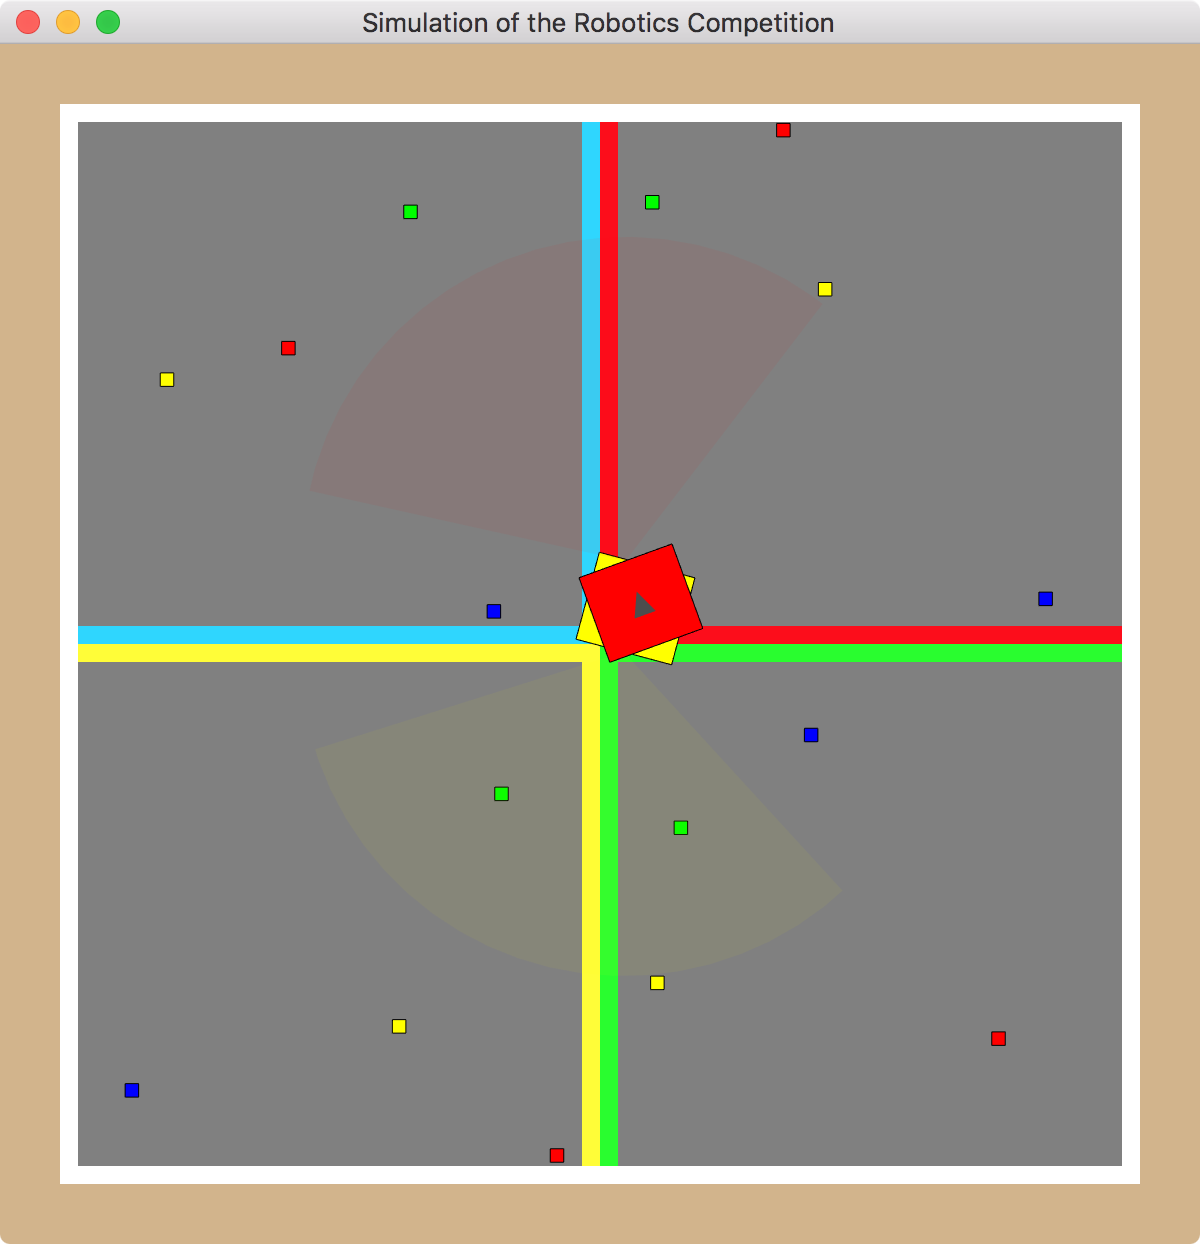
\includegraphics[width=.75\linewidth]{images/arena-3.png}
    \caption{Robots stuck on top of each other}
    \label{fig:arena-stuck-1}
  \end{subfigure}
  \begin{subfigure}{.5\textwidth}
    \centering
    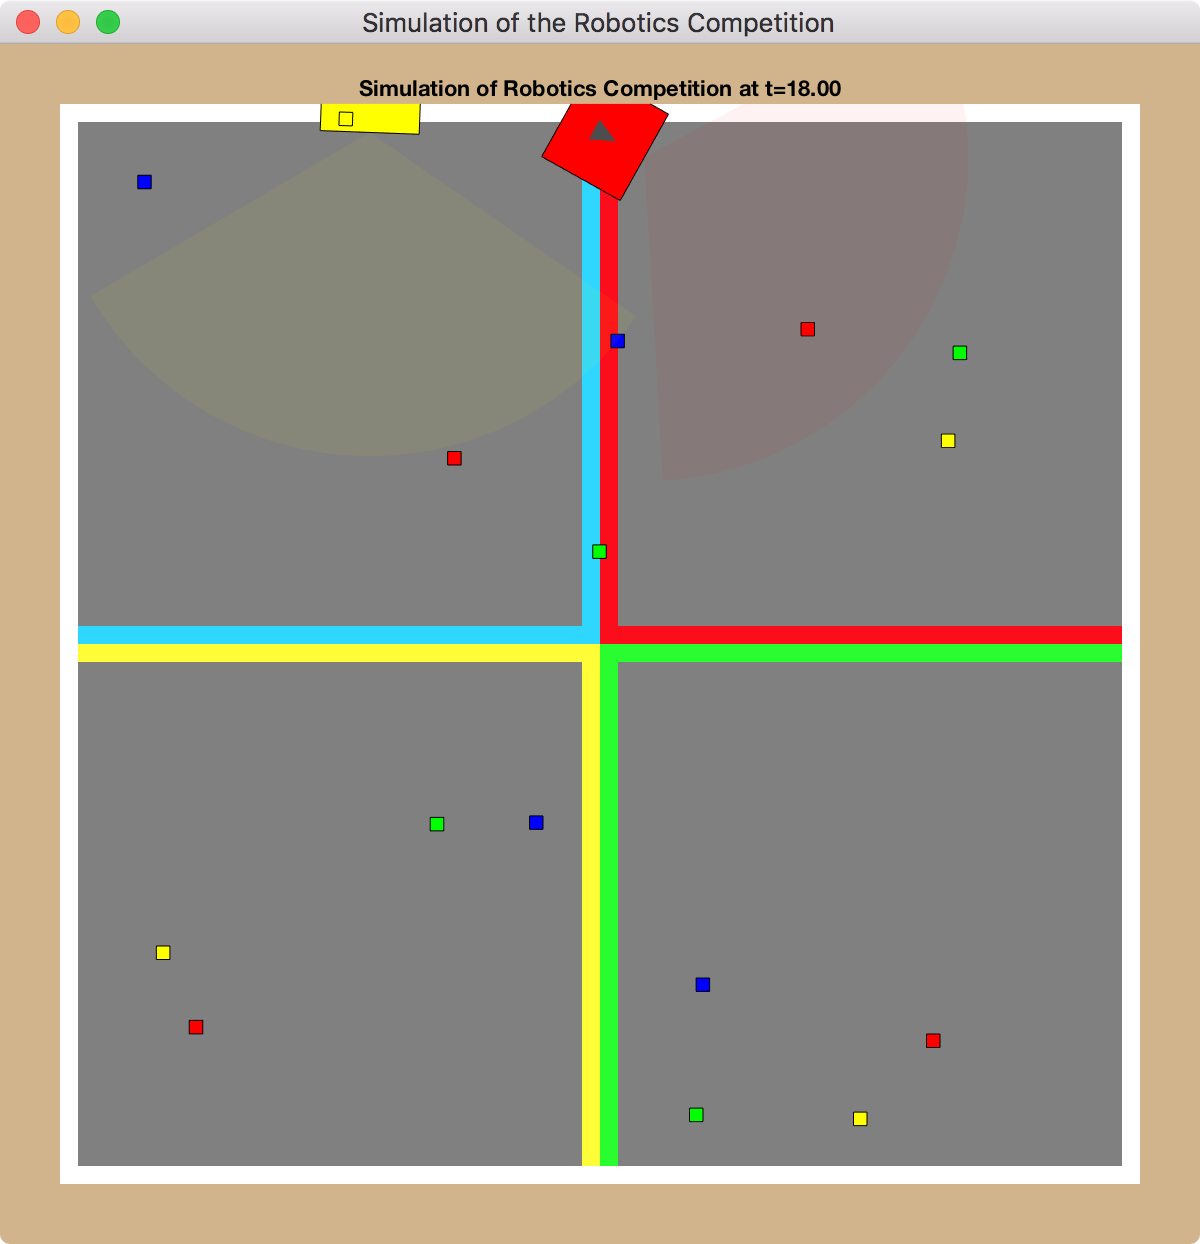
\includegraphics[width=.75\linewidth]{images/arena-4.png}
    \caption{Robots stuck outside the arena}
    \label{fig:arena-stuck-2}
  \end{subfigure}
  \caption{Two examples of robots that are stuck}
  \label{fig:arena-stuck}
\end{figure}

Another limitation of this implementation is that there can be some odd behavior at very low $dt$ values. For example, when $dt=1$ and the camera is turned off, robots will drive forward and then go entirely on top of each other. They will then get stuck spinning on top of each other indefinitely. This will also happen when they hit a boundary line. See Figure \ref{fig:arena-stuck-1} and Figure \ref{fig:arena-stuck-2} examples of this.

This implementation also only works for two robots. If I wanted to simulate more than two or just one robot, there would have to be significant code changes. Again, this decision was made for simplicity. The rules of the real competition assume that there are two robots in the arena (even if there is only one), and although I could have made it possible to simulate between 1 and 4 robots, it would have made the implementation more complex. I would have had to add a loop everywhere that there is references to each robot which definitely would have increased the complexity of the code.

Lastly, the biggest limitation of this implementation is that I only implemented one type of robot. In the real competition, all four robots were vastly different in the way that they were implemented. Some used the camera extensively, some (like ours) didn't use the camera at all. Also, three of the four robots used a mechanism to grab blocks one at a time and then bring them back to their home quadrant. Our robot used this collection mechanism, and the code relies on that substantially. It definitely would be non-trivial to implement robots of different types into this simulation. Although this is a substantial limitation in terms of the contest as a whole, this doesn't significantly impact the usefulness of this model as an evaluator of a robot that uses a sorting/collection mechanism. The main difference would be that with other robots they did focus on moving blocks out of their home quadrant and sabotaging their opponent, but that turned out to not be very significant during the actual competition.

\section{Code Validation}
There were two main strategies that I used to validate my code. First, I tested individual functions by manually building instances of the classes and running tests on specific functions. Second, I tested the system as a whole by running multiple random simulations using the same and differing parameters and looking at the results to make sure that things were running as expected.

\subsection{Individual Function Tests}
My first strategy for testing my code was to test individual methods by creating test instances of classes, manually setting parameters, and then testing the output of the methods using inputs where I had manually calculated the output.

For example, I validated the validity of the method \texttt{inFieldOfView} on the \texttt{Camera} class by creating a new instance of the \texttt{Camera} in the command window with the command \texttt{c = Camera(5, 135, 'red')}. Then, I tested the function with a number of different points. For example, the camera should be able to see a block 1 foot in front of it, so to test that I used the command \texttt{c.inFieldOfView(0,0,0,1,0)} which returned \texttt{1}, the expected output. Another test that I ran is for blocks that should not be in the field of view. One command I used to test that was \texttt{c.inFieldOfView(0,0,0,-1,0)} which returns \texttt{0}, since the block is behind the camera position.

I did a variety of similar tests on many methods as I was developing. I would check that the results were as expected, but I would also check to make sure error cases were also handled in ways that made sense. For example when testing the \texttt{Camera.getAngleOffCenter()} method (see Listing \ref{lst:getAngleOffCenter}), I tested that the function worked for values behind the camera as well as in front of it.

\subsection{Visual System Tests}
The second strategy that I used to validate my code's accuracy was by doing visual tests. After developing individual class methods (or even just small blocks of code within a method), I would run the simulation as a whole to see the result.

One place where I used this while developing was the \texttt{Camera.getAngleOffCenter()} method (see Listing \ref{lst:getAngleOffCenter}). This method is supposed to find the angle that the input point is off the center axis of the camera. In order to find this angle it creates two lines. One line is from the camera origin to 1 unit straight forward, and the other line is from the camera origin to the point of the object. We then calculate the angle between those two lines.

When developing this function, I wanted to make sure that the lines were accurate, since I was using some trigonometry in order to calculate a point. In order to do this, I added a debug flag (\texttt{Camera.Debug}) to the constants for the \texttt{Camera} class, and then plotted the two lines if the flag is set to \texttt{true}. I could then also print out the angle that is getting returned and do a visual check to make sure that the  angle matches what I would visually expect for the two lines. This allowed me to catch a subtle error which resulted in an error checking case being added to the function (see lines 17-20 in Listing \ref{lst:getAngleOffCenter}).

Another example where I used visual testing was in the block collection code. After adding code to check collect blocks as a robot runs over it, I confirmed the validity of this feature by adding code to display the blocks that a robot has in it's chamber, and testing that when a block got added to the chamber, it was also removed from the arena.

\section{Hypothesis Tests}
The following section describes some different hypothesis that I was able to test using the model. 

\subsection{Camera Effectiveness}
\textit{Hypothesis:} The addition of the camera allows robots to collect more blocks in a shorter amount of time. In general, the addition of the camera will increase the score for the robot as opposed to roaming randomly.

To test this hypothesis I ran a 5 simulations of the competition with the camera and without the camera and averaged the resulting scores for each robot. The average score across both robots in the simulations without the camera is 6, and the average score across both robots in the simulations \textit{with} the camera is 10. That means that robots with the camera scored the maximum amount of points possible ($(3 \times 10) - (2 \times 1) = 10$) in each round. This shows that there is a significant advantage to having the camera. 

\begin{figure}[hbt]
  \center
  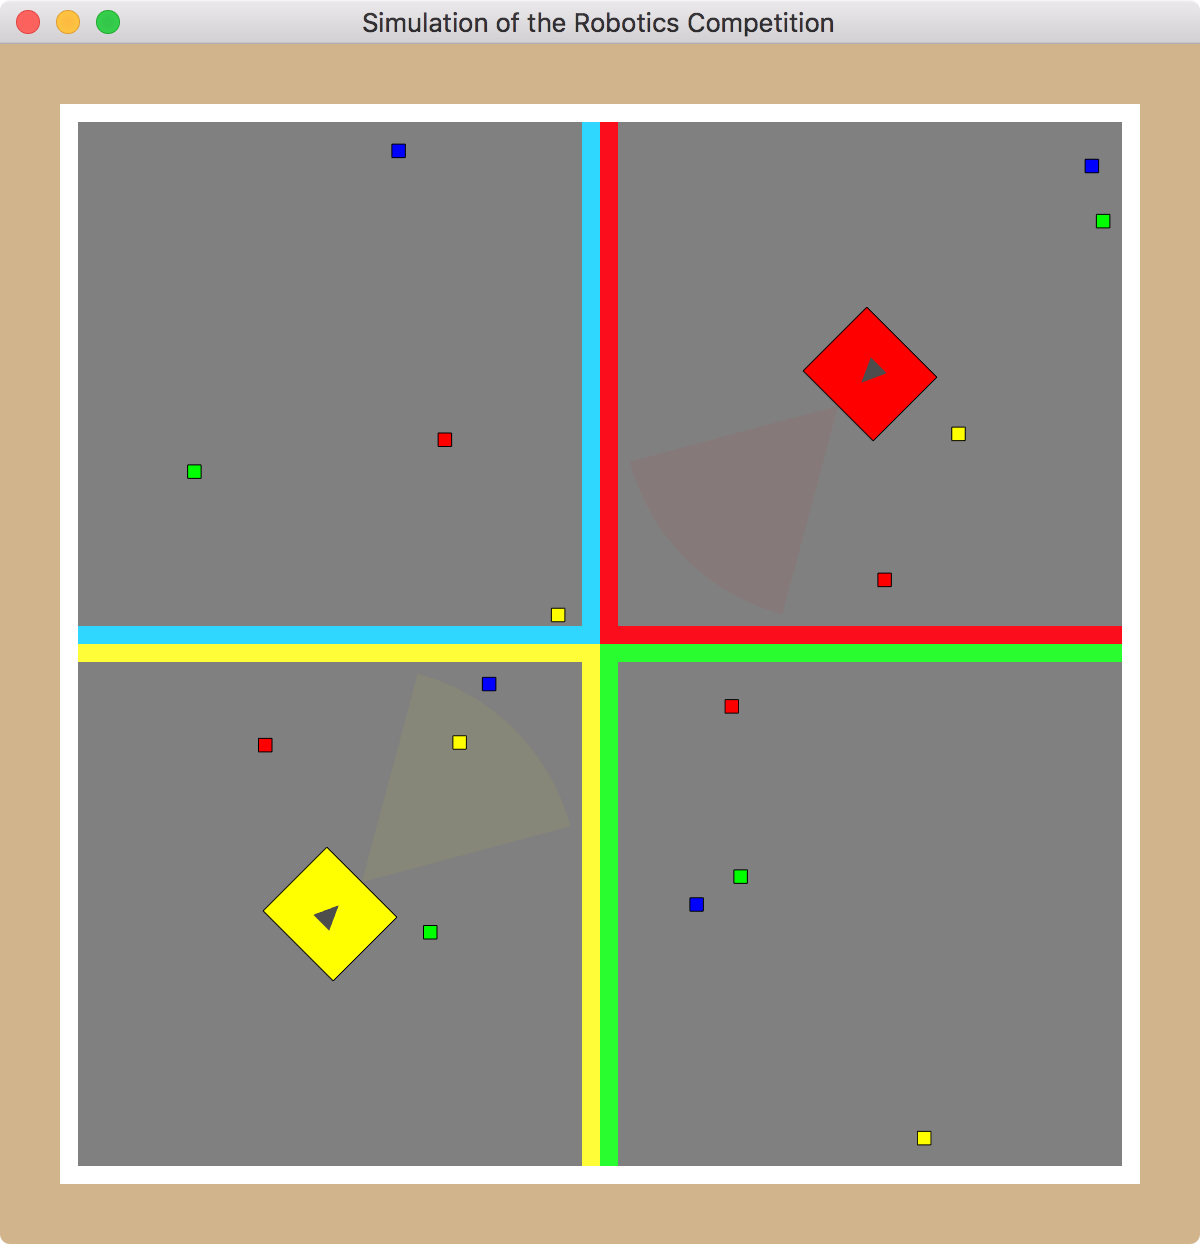
\includegraphics[width=0.45\textwidth]{images/arena-2.png}
  \caption{A screenshot at $t=0$ of the arena where both camera's are configured with a maximum view angle of 60\degree\ and maximum viewing distance of 3 ft.}
  \label{fig:arena-2}
\end{figure}

\subsection{Camera Field of View}
\textit{Hypothesis:} Because it is able to see more blocks on the arena, a camera with a wider and/or longer field of view will get a higher average score than one with a smaller and/or shorter field of view.

To test this hypothesis I ran 5 simulations for each of the following configurations: a 115\degree\ 3 ft. field of view, a 90\degree\ 3 ft. field of view, a 60\degree\ 3 ft. field of view, and a 60\degree\ 2 ft. field of view. The average score for each robot for each configuration, as well as the average score without the camera, is as follows.
\begin{itemize}
  \item 115\degree\ 3 ft. FOV: $(10+10+10+10+10+10+10+10+10+10)/10 = \textbf{10}$
  \item 90\degree\ 3 ft. FOV: $(10+9+7+10+10+10+4+10+10+10)/10 = \textbf{9}$
  \item 60\degree\ 3 ft. FOV: $(7+10+10+6+10+7+7+7+7+10)/10 = \textbf{8.1}$
  \item 60\degree\ 2 ft. FOV: $(7+10+7-2+9+3+4-2+10+4)/10 = \textbf{5}$
  \item No camera: $(10+9+7-2+1+7+4+9+9+7)/10 = \textbf{6}$
\end{itemize}

As you can see, the camera had a significant impact at higher angles and distances as expected. However, when the camera got down to 60\degree\ 2 ft., it actually performed worse than the runs without any camera.

One explanation for why the camera with this configuration did not perform better than the robot without the camera, is that the camera's field of view is almost entirely just directly in front of the robot. That is, if the robot was in a position where the block could be seen by the camera, the robot only had to drive forward to collect the block anyway. This can be seen in Figure \ref{fig:arena-2}.

Therefore, this evidence shows that the hypothesis is correct, that robots with a larger field of view are more likely to gain a higher score.

\subsection{Spin Angle}
\textit{Hypothesis:} The larger the range of spin angles that the robot is able to spin after hitting an obstacle, the more paths that it will be able to take, and the better score it would get. 

This hypothesis is not supported by evidence. I turned the camera off and ran 5 simulations each with the following configurations, shown in tuples representing the minimum and maximum spin angle: (45\degree, 180\degree), (0\degree, 180\degree), (0\degree, 90\degree), and (90\degree, 180\degree). The corresponding average scores for these configurations is 4.5, 4.1, 4.6, and 5 respectively. Since all of these values are within the range of 4 to 5 points, it doesn't seem that there is any advantage to having the robots spin with anything other than 90 to 180 degrees.

One type of configuration that I did not test was where the robot always spun at a specific angle (their min and max spin angle is equal). Since I had to use a low value for $dt$ in order to run the simulations in a reasonable amount of time, the robots were not able to spin at exactly the angle that they were supposed to. This would defeat the purpose of testing the spin angle.

\end{document}